\documentclass[10pt]{article}

\usepackage{listings}
\usepackage{color}
\usepackage{textcomp} % for upquote
\usepackage{etoolbox}
\usepackage[table]{xcolor}
\usepackage{multicol}
\usepackage{etoc}
\usepackage{hyperref}
\usepackage{graphicx}

% Requires package: color.
\definecolor{mediumgray}{rgb}{0.3, 0.4, 0.4}
\definecolor{mediumblue}{rgb}{0.0, 0.0, 0.8}
\definecolor{forestgreen}{rgb}{0.13, 0.55, 0.13}
\definecolor{darkviolet}{rgb}{0.58, 0.0, 0.83}
\definecolor{royalblue}{rgb}{0.25, 0.41, 0.88}
\definecolor{crimson}{rgb}{0.86, 0.8, 0.24}
\definecolor{Command}{RGB}{166, 127, 89}
\definecolor{Command2}{rgb}{0.25, 0.41, 0.88}
\definecolor{Digit}{RGB}{153, 0, 85}
\definecolor{FirstFn}{RGB}{25, 144, 184}
\definecolor{Gray}{gray}{0.9}
\newcommand\digitstyle{\color{Digit}}

\hypersetup{
	colorlinks=true,
	linkcolor=blue,
	filecolor=magenta,      
	urlcolor=blue,
	pdfpagemode=FullScreen,
}

%
% ECMAScript 2015 (ES6) definition by Gary Hammock
%

\lstdefinelanguage[ECMAScript2015]{JavaScript}[]{JavaScript}{
	morekeywords=[1]{await, async, case, catch, class, const, default, do,
		enum, export, extends, finally, from, implements, import, instanceof,
		let, static, super, switch, throw, try},
	morestring=[b]` % Interpolation strings.
}


%
% JavaScript version 1.1 by Gary Hammock
%
% Reference:
%   B. Eich and C. Rand Mckinney, "JavaScript Language Specification
%     (Preliminary Draft)", JavaScript 1.1.  1996-11-18.  [Online]
%     http://hepunx.rl.ac.uk/~adye/jsspec11/titlepg2.htm
%

\lstdefinelanguage{JavaScript}{	
	morekeywords=[1]{break, continue, delete, else, for, function, if, in,
		getDate, toDateString, toLocaleString, toString, toUTCString, getFullYear, log,
		get, getDate, getDay, getFullYear, getHours, getMilliseconds, getMinutes, getMonth, getSeconds, getTime,
		getTimezoneOffset, getUTCDate, getUTCDay, getUTCFullYear, getUTCHours, getUTCMilliseconds, getUTCMinutes, getUTCMonth, getUTCSeconds,
		new, return, this, typeof, var, void, while, with},
	% Literals, primitive types, and reference types.
	morekeywords=[2]{false, null, true, boolean, number, undefined,
		Array, Boolean, Date, Math, Number, String, Object},
	% Built-ins.
	morekeywords=[3]{eval, parseInt, parseFloat, escape, unescape},
	morekeywords=[4]{console},
	sensitive,
	morecomment=[s]{/*}{*/},
	morecomment=[l]//,
	morecomment=[s]{/**}{*/}, % JavaDoc style comments
	morestring=[b]',
	morestring=[b]"
}[keywords, comments, strings]


\lstalias[]{ES6}[ECMAScript2015]{JavaScript}

\lstdefinestyle{JSES6Base}{
	backgroundcolor=\color{white},
	basicstyle=\ttfamily,
	breakatwhitespace=false,
	breaklines=true,
	captionpos=b,
	columns=fullflexible,
	commentstyle=\color{mediumgray}\upshape,
	emph={},
	emphstyle=\color{crimson},
	extendedchars=true,  % requires inputenc
	fontadjust=true,
	frame=single,
	identifierstyle=\color{black},
	keepspaces=true,
	keywordstyle=\color{mediumblue},
	keywordstyle={[2]\color{darkviolet}},
	keywordstyle={[3]\color{royalblue}},
	keywordstyle={[4]\color{FirstFn}},
	numbers=left,
	numbersep=5pt,
	numberstyle=\tiny\color{black},
	numberfirstline=true,
	numberblanklines=true,
	rulecolor=\color{black},
	showlines=true,
	showspaces=false,
	showstringspaces=false,
	showtabs=false,
	stringstyle=\color{forestgreen},
	tabsize=2,
	title=\lstname,
	upquote=true,  % requires textcomp	
}

\lstset{
	language={ES6},
	literate=
		{<=}{{\textcolor{Command}{<=}}}1
		{>=}{{\textcolor{Command}{>=}}}1
		{=>}{{\textcolor{Command2}{=>}}}1
		{0}{{{\ProcessDigit{0}}}}{1}
		{1}{{{\ProcessDigit{1}}}}{1}
		{2}{{{\ProcessDigit{2}}}}{1}
		{3}{{{\ProcessDigit{3}}}}{1}
		{4}{{{\ProcessDigit{4}}}}{1}
		{5}{{{\ProcessDigit{5}}}}{1}
		{6}{{{\ProcessDigit{6}}}}{1}
		{7}{{{\ProcessDigit{7}}}}{1}
		{8}{{{\ProcessDigit{8}}}}{1}
		{9}{{{\ProcessDigit{9}}}}{1}
}

\lstdefinestyle{ES6}{
	language=ES6,
	style=JSES6Base
}

\makeatletter
\newcommand{\ProcessDigit}[1]
{%
	\ifnum\lst@mode=\lst@Pmode\relax%
	{\digitstyle #1}%
	\else
	#1%
	\fi
}
\makeatother

\begin{document}
	
\tableofcontents

\newpage

\section{Function}

\vbox{A JavaScript function is a block of code designed to perform a particular task. }

\begin{lstlisting}[style=ES6, caption={function}]
function echo() {
	console.log("Hello, JavaScript!");
}
\end{lstlisting}

\subsection{Calling functions}

\vbox{The function that makes the call is known as the calling function.}

\begin{lstlisting}[style=ES6, caption={Calling functions}]
function echo() {
	console.log("Hello, JavaScript!");
}

echo(); // Calling functions
"Hello, JavaScript!"
\end{lstlisting}

\subsection{Arrow functions}

\vbox{An arrow function expression (previously, and now incorrectly known as \textbf{fat arrow function}) has a shorter syntax compared to function expressions and does not have its own this, arguments, super, or new.target. Arrow functions are always anonymous.}

\begin{lstlisting}[style=ES6, caption={Calling functions}]
const echo = () => console.log("Hello, JavaScript!");
\end{lstlisting}

\subsection{Named functions}

\vbox{function with name}

\newpage

\section{Date}

\vbox{JavaScript Date objects represent a single moment in time in a platform-independent format. Date objects contain a Number that represents milliseconds since 1 January 1970 UTC.}

\subsection{Times and Days}

\subsubsection{Times}
\begin{table}[h!]
	\centering
	\begin{tabular}{ r l }
		1 second & 1000 milli seconds \\
		\rowcolor{Gray}
		1 mintue & 60 seconds \\  
		1 hour & 60 minutes \\
		\rowcolor{Gray}
		1 day & 24 hours \\
		1 week & 7 days \\
		\rowcolor{Gray}
		1 month & 28 - 31 days \\
		1 year & 365-366 days
	\end{tabular}
	\caption{Times}
\end{table}

\begin{table}[h!]
	\centering
	\begin{tabular}{ r l }
		1 second & 1000 \\
		\rowcolor{Gray}
		1 mintue & 60 * 1000 \\  
		1 hour & 60 * 60 * 1000 \\
		\rowcolor{Gray}
		1 day & 24 * 60 * 60 * 1000 \\
		1 week & 7 * 24 * 60 * 60 * 1000 \\
		\rowcolor{Gray}
		1 month & (28 - 31) * 24 * 60 * 60 * 1000  \\
		1 year & (365-366) * 24 * 60 * 60 * 1000
	\end{tabular}
	\caption{Milli seconds in times}
\end{table}

\subsubsection{Days in months}
\hspace{1cm}
\begin{tabular}{r l}
	month & days \\ [0.5ex] 
	\hline\hline
	\rowcolor{Gray}
	January & 31 days \\ 
	February & 28 days in a common year and 29 days in leap years \\
	\rowcolor{Gray}
	March & 31 days \\
	April & 30 days \\
	\rowcolor{Gray}
	May & 31 days \\ 
	June & 30 days \\
	\rowcolor{Gray}
	July & 31 days \\
	August & 31 days \\
	\rowcolor{Gray}
	September & 30 days \\
	October & 31 days \\
	\rowcolor{Gray}
	November & 30 days \\
	December & 31 days \\
	\hline
\end{tabular}

\hspace{1cm}
\subsubsection{AM: Anti Meridiem, PM: Post Meridiem}

AM and PM both are Latin words, used in 12-hour clock system to represent Before Noon and After Noon respectively. They are also represented as A.M. and P.M. \\ \hspace{1cm}

AM expand as Anti Meridiem which means "before midday" and PM expand as Post Meridiem which means "after midday". \hspace{1cm}

\begin{figure}[h]
	\centering
	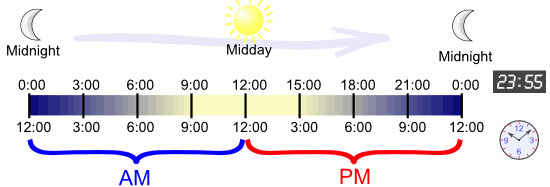
\includegraphics[width=1\linewidth]{day-am-pm}
	\caption{AM PM diagram}
	\label{fig:day-am-pm}
\end{figure}

\hspace{1cm}

\subsection{Create date instance}
\begin{lstlisting}[style=ES6, caption={Date instance}]
const date = new Date();
\end{lstlisting}

\subsection{Date string type methods}
\begin{lstlisting}[style=ES6, caption={Output of Date}]
const date = new Date();
console.log(date);
// Output - type: date object
// Sun Mar 20 2022 23:40:17 GMT+0530 (India Standard Time)
\end{lstlisting}

\begin{lstlisting}[style=ES6, caption={Date to String}]
const date = new Date();
const dateToStringMethod = date.toString();
console.log(dateToStringMethod);
// Output - type: string
'Sun Mar 20 2022 23:40:17 GMT+0530 (India Standard Time)'
\end{lstlisting}

\begin{lstlisting}[style=ES6, caption={Date to Date String}]
const date = new Date();
const dateToDateStringMethod = date.toDateString();
console.log(dateToDateStringMethod);
// Output - type: string
'Sun Mar 20 2022'
\end{lstlisting}

\begin{lstlisting}[style=ES6, caption={Date to Local String}]
const date = new Date();
const dateToLocalStringMethod = date.toLocaleString();
console.log(dateToLocalStringMethod);
// Output - type: string
'3/20/2022, 11:40:17 PM'
\end{lstlisting}

\begin{lstlisting}[style=ES6, caption={Date to UTC String}]
const date = new Date();
const dateToUTCStringMethod = date.toUTCString();
console.log(dateToUTCStringMethod);
// Output - type: string
'Sun, 20 Mar 2022 18:10:17 GMT'
\end{lstlisting}

\subsection{Date methods}

\begin{multicols}{2}
\begin{center}
Month \textbf{name} and its \textbf{index/value}
\newline
\newline
	\begin{tabular}{|cl|}
		\hline
		\textbf{Index/Value} & \textbf{Month} \\
		\hline
		0 & January \\
		\hline
		1 & February \\
		\hline
		2 & March \\
		\hline
		3 & April \\
		\hline
		4 & May \\
		\hline
		5 & June \\
		\hline
		6 & July \\
		\hline
		7 & August \\
		\hline
		8 & September \\
		\hline
		9 & October \\
		\hline
		10 & November \\
		\hline
		11 & December \\
		\hline
		\hline
	\end{tabular}
\end{center}
\columnbreak
\begin{center}
	Days \textbf{name} and its \textbf{index/value}
\end{center}
\begin{center}
	\begin{tabular}{|cl|}
		\hline
		\textbf{Index/Value} & \textbf{Day} \\
		\hline
		0 & Monday \\
		\hline
		1 & Tuesday \\
		\hline
		2 & Wednesday \\
		\hline
		3 & Thursday \\
		\hline
		4 & Friday \\
		\hline
		5 & Saturday \\
		\hline
		6 & Sunday \\
		\hline
		\hline
	\end{tabular}
\end{center}
\end{multicols}

\begin{lstlisting}[style=ES6, caption={Date methods - I}]
// DATE: YYYY-MM-DD: 2022-03-20
const date = new Date();
const currentDate = date.getDate();
console.log(currentDate);
// Output - type: number
// current date of month
20

const year = date.getFullYear();
console.log(year);
// Output - type: number
// current year
2022

const month = date.getMonth();
console.log(month);
// Output - type: number
// current month
// month start with 0
2

const day = date.getDay();
console.log(day);
// Output - type: number
// current day
// day start with 0
6
\end{lstlisting}
\begin{lstlisting}[style=ES6, caption={Date methods - II}]
// Mon Mar 21 2022 12:45:51 GMT+0530 (India Standard Time)
const date = new Date();
const hours = date.getHours();
console.log(hours);
// Output - type: number
// current hour/hours
12

const mintues = date.getMinutes();
console.log(mintues);
// Output - type: number
// current mintues
45

const seconds = date.getSeconds();
console.log(seconds);
// Output - type: number
// current seconds
51

const milliSeconds = date.getMilliseconds();
console.log(milliSeconds);
// Output - type: number
// current milli seconds
236

const time = date.getTime();
console.log(time);
// Output - type: number
// current time
1647846951236

const timeZoneOffset = date.getTimezoneOffset();
console.log(timeZoneOffset);
// Output - type: number
// current time zone offset
-330
\end{lstlisting}

\subsection{Date methods - UTC}

UTC - Universal Coordinated Time

\begin{lstlisting}[style=ES6, caption={UTC Date methods - I}]
// DATE: YYYY-MM-DD: 2022-03-20
const date = new Date();
const currentUTCDate = date.getUTCDate();
console.log(currentUTCDate);
// Output - type: number
// current date of month
20

const yearUTC = date.getUTCFullYear();
console.log(yearUTC);
// Output - type: number
// current year
2022

const monthUTC = date.getUTCMonth();
console.log(monthUTC);
// Output - type: number
// current month
// month start with 0
2

const dayUTC = date.getUTCDay();
console.log(dayUTC);
// Output - type: number
// current day
// day start with 0
6
\end{lstlisting}
\begin{lstlisting}[style=ES6, caption={UTC Date methods - II}]
// Mon Mar 21 2022 16:47:01 GMT+0530 (India Standard Time)
const date = new Date();
const hoursUTC = date.getUTCHours();
console.log(hoursUTC);
// Output - type: number
// current hour(s)
11

const mintuesUTC = date.getUTCMinutes();
console.log(mintuesUTC);
// Output - type: number
// current mintue(s)
17

const secondsUTC = date.getUTCSeconds();
console.log(secondsUTC);
// Output - type: number
// current second(s)
1

const milliSecondsUTC = date.getUTCMilliseconds();
console.log(milliSecondsUTC);
// Output - type: number
// current milli second(s)
666
\end{lstlisting}

\subsection{Date methods - static}

\subsubsection{now()}

A Number representing the milliseconds elapsed since the UNIX epoch

\begin{lstlisting}[style=ES6, caption={Date methods - static now}]
	Date.now();
	// Output - type: number
	// 1647864341072
\end{lstlisting}

\subsection{Date methods - Set}

\subsubsection{setFullYear}
\begin{itemize}
\color{red}
\item[year] required
\color{forestgreen}
\item[month] optional

\item[date] optional
\end{itemize}
\begin{lstlisting}[style=ES6, caption={Date methods - full year}]
const date = new Date();
// Mon Mar 21 2022 17:06:30 GMT+0530 (India Standard Time)

// set year(s)
date.setFullYear(2025)
// Fri Mar 21 2025 17:06:30 GMT+0530 (India Standard Time)
\end{lstlisting}

\subsubsection{setMonth}
\begin{itemize}
\color{red}
\item[month] required
\color{forestgreen}

\item[date] optional
\end{itemize}

set month: 0(January) - 11(December)

\begin{lstlisting}[style=ES6, caption={Date methods - month(s)}]
const date = new Date();
// Mon Mar 21 2022 17:10:44 GMT+0530 (India Standard Time)

// set month(s)
date.setMonth(1)
// Mon Feb 21 2022 17:10:44 GMT+0530 (India Standard Time)
\end{lstlisting}

\subsubsection{setDate}
\begin{itemize}
\color{red}
\item[date] required
\end{itemize}

set date: 1 - 31

feb month - 28, 29(leap year)

\begin{lstlisting}[style=ES6, caption={Date methods - date(s)}]
const date = new Date();
// Mon Mar 21 2022 17:11:44 GMT+0530 (India Standard Time)

// set date(s)
date.setDate(20)
// Sun Mar 20 2022 17:11:44 GMT+0530 (India Standard Time)
\end{lstlisting}

\subsubsection{setHours}
\begin{itemize}
	\color{red}
	\item[hours] required
	\color{forestgreen}
	
	\item[mintues] optional
	
	\item[seconds] optional
	
	\item[milli seconds] optional
\end{itemize}

set hours: 0 - 23

\begin{lstlisting}[style=ES6, caption={Date methods - hour(s)}]
	const date = new Date();
	// Mon Mar 21 2022 17:19:51 GMT+0530 (India Standard Time)
	
	// set hour(s)
	date.setHours(5)
	// Mon Mar 21 2022 05:19:51 GMT+0530 (India Standard Time)
\end{lstlisting}

\subsubsection{setMinutes}
\begin{itemize}
	\color{red}
	\item[mintues] required
	\color{forestgreen}

	\item[seconds] optional
	
	\item[milli seconds] optional
\end{itemize}

set mintues: 0 - 59

\begin{lstlisting}[style=ES6, caption={Date methods - mintue(s)}]
	const date = new Date();
	// Mon Mar 21 2022 17:23:53 GMT+0530 (India Standard Time)
	
	// set mintue(s)
	date.setMinutes(10)
	// Mon Mar 21 2022 17:10:53 GMT+0530 (India Standard Time)
\end{lstlisting}

\subsubsection{setSeconds}
\begin{itemize}
	\color{red}
	\item[seconds] required
	\color{forestgreen}
	
	\item[milli seconds] optional
\end{itemize}

set seconds: 0 - 59

\begin{lstlisting}[style=ES6, caption={Date methods - second(s)}]
	const date = new Date();
	// Mon Mar 21 2022 17:25:50 GMT+0530 (India Standard Time)
	
	// set second(s)
	date.setSeconds(10)
	// Mon Mar 21 2022 17:25:10 GMT+0530 (India Standard Time)
\end{lstlisting}

\subsubsection{setMilliSeconds}
\begin{itemize}
	\color{red}
	\item[milli seconds] required
\end{itemize}

set milli seconds: 0 - 999

\begin{lstlisting}[style=ES6, caption={Date methods - milli second(s)}]
	const date = new Date();
	// date.getTime() - 1647863993085
	
	// set milli second(s)
	date.setMilliseconds(500)
	// 1647863993500
\end{lstlisting}

\subsubsection{setTime}
\begin{itemize}
	\color{red}
	\item[times] required
\end{itemize}

set milli seconds since January 1,  1970

\begin{lstlisting}[style=ES6, caption={Date methods - time}]
	const date = new Date();
	// Mon Mar 21 2022 17:32:27 GMT+0530 (India Standard Time)
	// date.getTime() - 1647863993085
	
	// set time
	date.setTime(1000)
	// 1000
	// Thu Jan 01 1970 05:30:01 GMT+0530 (India Standard Time)
\end{lstlisting}

\begin{thebibliography}{9}
\bibitem{date1}
\href{https://momentjs.com/}{momentjs}: \textbf{Parse}, \textbf{validate}, \textbf{manipulate}, and \textbf{display} \emph{dates} and \emph{times} in JavaScript. [\href{https://bundlephobia.com/package/moment}{bundle details}]
	
\bibitem{date2}
\href{https://date-fns.org/}{date-fns}: date-fns provides the most comprehensive, yet simple and consistent toolset for manipulating \textbf{JavaScript dates} in a \textbf{browser} \& \textbf{Node.js}. [\href{https://bundlephobia.com/package/date-fns}{bundle details}]

\bibitem{date3}
\href{https://day.js.org/}{Day.js}: Fast 2kB alternative to Moment.js with the same modern API [\href{https://bundlephobia.com/package/dayjs}{bundle details}]

\bibitem{date4}
\href{https://moment.github.io/luxon/#/}{luxon}: A powerful, modern, and friendly wrapper for JavaScript dates and times. [\href{https://bundlephobia.com/package/luxon}{bundle details}]

\end{thebibliography}

\textbf{Trends} - date-fns vs dayjs vs luxon vs moment

\url{https://www.npmtrends.com/date-fns-vs-luxon-vs-moment-vs-dayjs}

\end{document}